\subsection{Totale Korrektheit}
\label{sec:Kap-11-2-5}

\minisec{Terminierung von Schleifen}

Wir haben in den Beispielen oben bereits gezeigt, dass die jeweiligen Schleifen tatsächlich terminieren. Dazu haben wir Abstiegsfunktionen angegeben, also Funktionen mit Argumenten aus den Variablen, die im Schleifenrumpf modifiziert werden können. Die Werte einer Abstiegsfunktion dürfen nicht beliebig klein werden, und sie müssen bei jedem Schleifendurchlauf kleiner werden. Typischerweise wird bei dem kleinstmöglichen Wert die Schleife verlassen, aber oftmals kann die Schleife auch bei größeren Werten verlassen werden.

Aber Vorsicht, die fortgesetzte Halbierung einer Zahl führt auch zu einer immer kleiner werdenden Zahl, ohne dass die 0 jemals erreicht wird. Deshalb betrachtet man nur ganzzahlige Abstiegsfunktionen, \dasHeisst der Wert reduziert sich bei jedem Schleifendurchlauf um wenigstens 1.

Abstiegsfunktionen sind nicht immer offensichtlich oder leicht zu finden. Betrachten Sie als Beispiel folgendes Programm:

\vspace{\baselineskip} %%% für Druck

\begin{algorithm}[H]
	\caption{$n+1$-Programm}
	\label{algo:n_plus_1_programm}
	
	\vspace{2mm} %%% für Druck
	\vspace{\baselineskip}
	
	\KwData{Eingabe: $n > 0$}
	\KwResult{Ausgabe: $m$}
	
	\vspace{2mm} %%% für Druck
	\vspace{\baselineskip}
	
	$m = 0$\;
	
	\vspace{2mm} %%% für Druck
	\vspace{\baselineskip}

	\While{$n > 1$}{
		\eIf{\text{odd}($n$)}{
			$n = n + 1$
		}{
			$n = n / 2$
		}
		$m = m + 1$
	}
	\;
	
	\vspace{2mm} %%% für Druck
	\vspace{\baselineskip}
	
	\Return{$m$}
	\vspace{2mm} %%% für Druck
	\vspace{\baselineskip}
\end{algorithm}

\pagebreak %%% für Druck

Auf die Ausgabe $m$ kommt es hier gar nicht an, sondern uns interessiert nur, dass und warum die Schleife sicher irgendwann verlassen wird. Für verschiedene Anfangswerte ($n = 5, 12, 13$) erhalten wir die folgenden Zahlenfolgen für $n$:

\begin{center}
	$5, 6, 3, 4, 2, 1$ \\
	$12, 6, 3, 4, 2, 1$ \\
	$13, 14, 7, 8, 4, 2, 1$
\end{center}

Aber was steigt hier ab?

Bevor Sie sich die Lösung ansehen, versuchen Sie doch selbst herauszufinden, wie eine für dieses Programm passende Abstiegsfunktion aussehen könnte.

$\vdots$

Und hier ist eine mögliche Lösung:

$$ f: \{1,2,3, \ldots\} \rightarrow \{0,1,2, \ldots \}, \quad f(n) =
\begin{cases}
	0 & \text{für } n = 1 \\
	n - 1 & \text{für } n \text{ gerade} \\
	n + 1 & \text{für } n \text{ ungerade, } n > 1
\end{cases}$$


Die Folge der Funktionswerte für die Argumente $1,2,3,4,5,6,7,8, \ldots$ lautet damit

$$ 0,1,4,3,6,5,8,7, \ldots $$

Nun ist zu zeigen, dass es sich tatsächlich um eine Abstiegsfunktion handelt, bei jedem Schleifendurchlauf der Funktionswert also um wenigstens 1 kleiner wird. Zu beachten ist, dass die Schleife für $n= 1$ verlassen wird, wir also nur die Fälle $n > 1$ betrachten müssen.

\vspace{\baselineskip}

\begin{addmargin}[25pt]{25pt}
\begin{labeling}{{\textbf{xx. Fall:}}} % "xx. Fall" ist hier nur ein Platzhalter
	\item[\textbf{1. Fall:}] $n$ ist eine ungerade Zahl \\
		Dann ist $n \geq 3$. $n$ wird um 1 erhöht. Nach Konstruktion von $f$ gilt $f(n+1) = n = f(n)-1$, der Wert von $f(n)$ wird also kleiner.
	\item[\textbf{2. Fall:}] $n$ ist eine gerade Zahl, $n/2$ ist ebenfalls eine gerade Zahl \\
		$n$ wird im Schleifendurchlauf halbiert. Es gilt $f (n) = n-1 $ und $f(n/2) = n/2 -1$. Der Wert von $f(n)$ wird also um $n/2$ kleiner.
	\item[\textbf{3. Fall:}] $n$ ist eine gerade Zahl, $n/2$ ist eine ungerade Zahl, $n \neq 2$ \\
		Es gilt $f(n) = n-1$ und $f(n/2) = n/2 +1$. Der Wert von $f(n)$ wird also um $n/2 - 2$ reduziert. Dieser Wert ist positiv, da nach Voraussetzung $n\geq 6$ gilt ($n=2$ ist ausgeschlossen, für $n= 4$ ist $n/2$ gerade).
	\item[\textbf{4. Fall:}] $n=2$ \\
		Dann gilt $f(n)= f(2)= 1$. $n$ wird um 1 reduziert und 
		\linebreak
		$f(1) = 0<1$.
\end{labeling}
\end{addmargin}

\vspace{\baselineskip}

Der Funktionswert $f(n)$ wird also in jedem Fall bei jedem Schleifendurchlauf um wenigstens 1 reduziert, weshalb $f$ eine hier passende Abstiegsfunktion darstellt.

In den meisten Fällen sind Abstiegsfunktionen allerdings offensichtlicher, aber nicht immer! Vielleicht macht es Ihnen Spaß, Variationen dieses Beispiels zu untersuchen. Was gilt, wenn ungerade $n$ nicht um 1, sondern um 3 erhöht werden (und gerade $n$ weiterhin halbiert werden)? Eine andere Variation: Bei ungeradem $n$ wird $n$ durch $3n + 1$ ersetzt. Für einen Anfangswert $n=17$ entsteht dann die Zahlenfolge

$$ 17, 52, 26, 13, 40, 20, 10, 5, 16, 8, 4, 2, 1$$

Aber endet diese Folge für jeden beliebigen Anfangswert von $n$, und wie lautet eine entsprechende Abstiegsfunktion? Wenn Sie hier eine akzeptable Antwort finden, werden Sie reich und berühmt. Es handelt sich nämlich um das bekannte Collatz-Problem 
\marginline{Collatz-Problem}
(auch $(3n+1)$-Problem genannt). Man hat weder jemals eine Anfangszahl gefunden, für die diese Schleife nicht terminiert, noch eine Abstiegsfunktion oder irgendeinen anderen Beweis dafür, dass die Schleife immer terminiert.

\minisec{Terminierung bei Rekursion}

Für nicht terminierende Programme braucht man nicht notwendigerweise Schleifen, die sich als Endlosschleifen herausstellen! Derselbe Effekt eines immer weiter laufenden Programms, das nicht zum Ende kommt, taucht auch auf, wenn sich ein Programm (oder eine programmierte Funktion) immer wieder selbst aufruft. Unser letztes Beispiel aus Algorithmus~\ref{algo:n_plus_1_programm} könnte man auch rekursiv programmieren durch

\vspace{\baselineskip}

\begin{algorithm}[H]
	\caption{fun function}
	\label{algo:fun_function}
	
	\vspace{\baselineskip}
	
	\KwData{Eingabe: $n$}
	\KwResult{Ausgabe: None}
	
	\vspace{\baselineskip}
	
	\SetKwFunction{Function}{fun}
	\SetKwProg{Fn}{Function}{:}{end}
	
	\vspace{\baselineskip}
	
	\Fn{\Function{$n$}}{
		\eIf{$n = 1$}{
			\text{stopp}
		}{
			\eIf{\text{odd}($n$)}{
				$\Function(n+1)$
			}{
				$\Function(n/2)$
			}
		}
	}
	
	\vspace{\baselineskip}
\end{algorithm}

\vspace{\baselineskip}

Hätte die Funktion nicht wenigstens einen Fall, in dem sie sich nicht wieder selbst aufruft (hier der Fall $n=1$), dann würden die Selbstaufrufe unweigerlich kein Ende finden. Aber auch wenn es die Möglichkeit eines Endes gibt, ist noch nicht gewährleistet, dass dieses Ende jemals erreicht wird. Notwendig dafür ist, dass das Argument, mit dem die Funktion sich selbst aufruft, kleiner wird, oder eine weniger komplexe Struktur besitzt oder dass es irgendeinen anderen Grund gibt, dass die Abbruch\-bedingung jemals erreicht wird. Hier kann man wie bei Schleifen eine Abstiegsfunktion\footnote{Vorsicht, die doppelte Verwendung von „Funktion“ als Programmelement einerseits und als Abstiegsfunktion andererseits mag verwirren!} $f$ verwenden. Wenn die (Programm-)Funktion mit Argument $n$ aufgerufen wird, darf sie sich selbst nur mit Argumenten $n'$ aufrufen, für die $f(n') < f(n)$ gilt. Die Abstiegsfunktion muss ganzzahlige Werte haben, und diese Werte dürfen nicht beliebig klein werden. Bei einem bestimmten kleinen Wert für $f(n)$ ruft sich die (Programm-)Funktion nicht wieder selbst auf, sondern terminiert; dann kann die aufrufende Instanz der Funktion ebenfalls terminieren, usw.

Bei rekursiven Aufrufen muss man also besonders aufpassen, dass die verwendeten Argumente kleiner werden. Woran aber erkennt man rekursive Aufrufe? Der offensichtliche und einfachste Fall ist, dass sich ein Programm, ein Unterprogramm oder eine Funktion selbst aufruft, der Name (des Programms / der Funktion) kommt also im Rumpf (desselben / derselben) wieder vor. Aber Rekursion entsteht auch, wenn zwei Programme sich abwechselnd gegenseitig aufrufen.

Hierzu ein Beispiel: Ein besonders fauler Programmierer soll ein Programm schreiben, das für eine eingegebene Zahl $n>0$ bestimmt, ob $n$ gerade ist. Er weiß, dass sein Kollege dieselbe Aufgabe für ungerade Zahlen zu lösen hat. Also ruft sein Programm $\text{even} (n)$ für $n>1$ das Programm $\text{odd} (n-1)$ auf und gibt $true$ aus, wenn $\text{odd}(n-1)$ \emph{false} ergibt, und umgekehrt. Für die Eingabe $n=1$ wird einfach \emph{false} ausgegeben.

Der Kollege macht es allerdings nicht anders. Sein Programm $\text{odd}(n)$ ruft bei Eingabe $n>1$ das Programm $\text{even} (n-1)$ auf und negiert ebenfalls das Ergebnis. Bei Eingabe $n=1$ wird \emph{true} ausgegeben.

Man sieht leicht, dass hier $\text{even}$ und $\text{odd}$ sich zwar nicht jeweils selbst aufrufen, mittelbar jedoch schon. Das besonders ineffiziente Programm terminiert für jedes $n$, und dies lässt sich mit der Abstiegsfunktion $f(n) = n$ auch beweisen.

Dasselbe Paar fauler Programmierer soll nun die Sinus- bzw. Cosinuswerte für eine eingegebene Zahl bestimmen. Der erste verlässt sich auf den zweiten und weiß, dass $\sin (\alpha) = \cos (90^\circ - \alpha)$ gilt. Sein Programm ruft also das Cosinusprogramm mit dem entsprechend modifizierten Argument auf. Der zweite Programmierer ist wieder nicht besser, kennt das Gesetz $\cos (\alpha) = \sin(90^\circ - \alpha)$, und überlässt die tatsächliche Berechnung der trigonometrischen Funktion seinem Kollegen. Es ist leicht zu sehen, dass sich die Programme für jeden Eingabewert gegenseitig mit immer wieder denselben Werten aufrufen, doch nie zu einem Ende kommen.

Doch es kann noch komplizierter kommen: Ein Programm $A$ kann ein Programm $B$ aufrufen, $B$ ruft $C$ auf, $C$ ruft $D$ auf und $D$ ruft wieder $A$ auf. Dies können die Programme im Kreis endlos machen, und das gesamte Programm terminiert nicht. Nun kann man den beteiligten Programmen natürlich nicht ohne Weiteres ansehen, ob sie -- und wenn, dann mit welchem Argument -- andere Programme überhaupt aufrufen, selbst wenn ein entsprechender Aufrufbefehl im Programmtext vorkommt. Aber umgekehrt gilt: Nur wenn diese Aufrufbefehle vorkommen, gibt es die Möglichkeit nicht endender rekursiver Aufrufe und damit die Notwendigkeit zu begründen, dass die Aufrufe irgendwann einmal enden. Wie beschrieben, kann dies mit einer Abstiegsfunktion geschehen, die bei vielen beteiligten Programmen recht kompliziert sein kann.

Wenn ein Programm sich selbst aufruft, sprechen wir von \emph{direkter Rekursion}. 
\marginline{direkte Rekursion\\ \vspace{2mm} indirekte Rekursion}
Situationen, wie hier beschrieben, in denen ein Programm sich nicht unmittelbar selbst aufruft, aber schließlich doch aufgerufen wird, heißen \emph{indirekte Rekursion}.

Wie bekommt man heraus, ob eine indirekte Rekursion vorliegt? $A$ ruft $B$ und $E$ auf, $B$ ruft $C$ und $D$ auf auf, $C$ ruft nichts auf, $D$ ruft $E$ auf und $E$ ruft $B$ und $C$ auf. Haben Sie den Überblick behalten? Jedenfalls kann im allgemeinen die Situation unübersichtlich sein, und eine indirekte Rekursion kann leicht übersehen werden. Hier helfen uns Graph-Algorithmen, wie wir nun zum Abschluss des Kapitels zeigen werden.

Sei $M$ eine Menge von Programmen. Wir definieren eine Relation $ \text{call} \colon M \to M$ durch $(X, Y) \in \text{call}$, wenn in $X$ ein Aufruf von $Y$ vorkommt. Die Menge $M$ und die Relation $\text{call}$ können als gerichteter Graph dargestellt werden, mit Knotenmenge $M$ und gerichteten Kanten $\text{call}$. Wir nennen diesen Graph \emph{Aufrufgraph}. 
\marginline{Aufrufgraph}
Für das oben textuell genannte Beispiel sieht der Aufrufgraph so aus:

\begin{figure}[h]
	\centering
	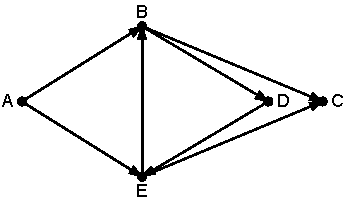
\includegraphics[width=0.50\textwidth]{Bilder/Kapitel-11/Aufrufgraph.pdf}
	\caption{Aufrufgraph}
	\label{fig:aufrufgraph}
\end{figure}

Es liegt Rekursion vor, wenn der Graph \textit{Zyklen} enthält. Eine direkte Rekursion ist ein Zyklus $(X,X)$, also eine Kante von einem Knoten zu sich selbst. Eine indirekte Rekursion entspricht einem Zyklus größerer Länge. In unserem Beispiel finden wir $(B,D), (D, E), (E,B)$ als Zyklus, der die indirekte Rekursion beschreibt.

Ein Zyklus in einem gerichteten Graphen ist visuell selbsterklärend und formal \mbox{definiert} als Kantenfolge 
$$ (X_1, X_2), (X_2, X_3), \ldots , (X_{i-1}, X_{i}), (X_{i}, X_1),$$ 
wobei für $i=1$ die Folge nur aus der Kante (Schlinge) $(X_1, X_1)$ besteht.

Um indirekte Rekursion zu erkennen, muss also der Aufrufgraph ermittelt werden, und dieser muss auf Zyklen untersucht werden. Effiziente Algorithmen, die dies leisten, lernen Sie in anderen Modulen kennen.

\vspace{1.5cm}
ENDE.